\documentclass[../mathNotesPreamble]{subfiles}

\providecommand{\relscalefact}{1.4}
\begin{document}
\relscale{\relscalefact}
  \section{10.3: Isomorphisms of Graphs}

  %TODO define isomorphic (p713)
  \begin{defn*}
    Let $G$ and $G'$ be graphs with vertex sets $V(G)$ and $V(G')$ and edge sets $E(G)$ and $E(G')$, respectively. \textbf{$G$ is isomorphic to $G'$} if, and only if, there exist one-to-one correspondences $g: V(G)\to V(G')$ and $h: E(G) \to E(G')$ that preserve the edge-endpoint functions of $G$ and $G'$ in the sense that for each $v\in V(G)$ and $e\in E(G)$,
      \[v \textnormal{ is an endpoint of } e \Leftrightarrow g(v) \textnormal{ is an endpoint of } h(e).\]

    If $G$ and $G'$ are simple (no loops or parallel edges), then $G$ is isomorphic to $G'$ if, and only if, there exists $g: V(G)\to V(G')$ such that
      \[\set{u,v} \textnormal{ is an edge in } G \Leftrightarrow \set{g(u), g(v)} \textnormal{ is an edge in } G'.\]
  \end{defn*}
  \begin{ex*}
    Show that the following graphs are isomorphic:
    \begin{center}
      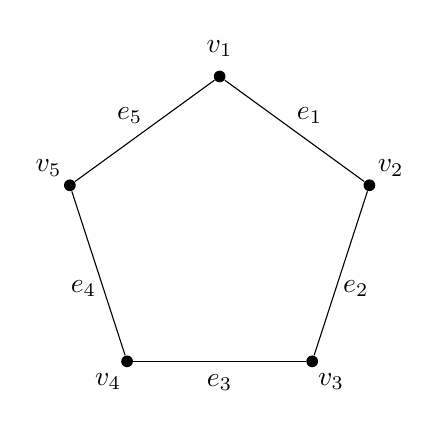
\begin{tikzpicture}[
        every node/.style={circle, fill=black, inner sep=1.5pt},
        edgeLbl/.style={fill=none, inner sep=1.5pt, pos=0.5},
      ]
        \foreach \steps/\text in {
          1/v_1,
          2/v_2,
          3/v_3,
          4/v_4,
          5/v_5}
          {
            \pgfmathsetmacro{\angle}{(1-\steps)*360/5+90};
            \draw (\angle:2 ) node[label=\angle:$\text$] (\text) {};
          }
        \draw (v_1) -- (v_2) node[edgeLbl, above right] {$e_1$};
        \draw (v_2) -- (v_3) node[edgeLbl, below right] {$e_2$};
        \draw (v_3) -- (v_4) node[edgeLbl, below] {$e_3$};
        \draw (v_4) -- (v_5) node[edgeLbl, below left] {$e_4$};
        \draw (v_5) -- (v_1) node[edgeLbl, above left] {$e_5$};
      \end{tikzpicture}
      \hspace*{25mm}
      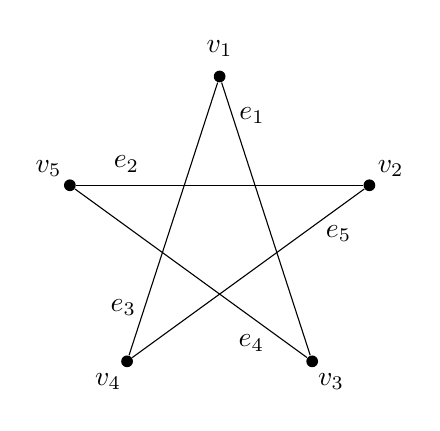
\begin{tikzpicture}[
        every node/.style={circle, fill=black, inner sep=1.5pt},
        edgeLbl/.style={fill=none, inner sep=1.5pt, pos=0.175},
      ]
        \foreach \steps/\text in {
          1/v_1,
          2/v_2,
          3/v_3,
          4/v_4,
          5/v_5}
          {
            \pgfmathsetmacro{\angle}{(1-\steps)*360/5+90};
            \draw (\angle:2 ) node[label=\angle:$\text$] (\text) {};
          }
        \draw (v_1) -- (v_3) node[edgeLbl, above right] {$e_1$};
        \draw (v_2) -- (v_4) node[edgeLbl, below right] {$e_5$};
        \draw (v_3) -- (v_5) node[edgeLbl, below left] {$e_4$};
        \draw (v_4) -- (v_1) node[edgeLbl, left] {$e_3$};
        \draw (v_5) -- (v_2) node[edgeLbl, above] {$e_2$};
      \end{tikzpicture}
    \end{center}
    \vspace*{\stretch{1}}
  \end{ex*}
  \pagebreak

  %TODO example 10.3.1
  \begin{ex*}
    Show that the following graphs are isomorphic:
    \vspace*{\baselineskip}

    \begin{minipage}{0.45\linewidth}
      \begin{center}
        \begin{tikzpicture}[
          node distance=10mm and 20mm,
          every node/.style={circle, fill=black, inner sep=1.5pt},
          edgeLbl/.style={fill=none, inner sep=1.5pt, pos=0.5},
        ]
          \node[label=180:$v_1$] (v1) {};
          \node[above right=of v1, label=0:$v_2$] (v2) {};
          \node[below right=of v1, label=0:$v_5$] (v5) {};
          \node[above right=10mm and 30 mm of v2, label=0:$v_3$] (v3) {};
          \node[below right=10mm and 30 mm of v5, label=0:$v_4$] (v4) {};
          %%
          \draw (v1) -- (v5) node[edgeLbl, below left] {$e_5$};
          \draw (v1) -- (v2) node[edgeLbl, above left] {$e_7$};
          \draw (v2) -- (v5) node[edgeLbl, right] {$e_6$};
          \draw (v3) to [bend right] node[edgeLbl, left] {$e_2$} (v4);
          \draw (v3) to [bend left] node[edgeLbl, right] {$e_3$} (v4);
          \draw (v1) edge [out=90, in=180] node[edgeLbl, above] {$e_1$} (v3);
          \draw (v1) edge [out=-90, in=180] node[edgeLbl, below] {$e_4$} (v4);
        \end{tikzpicture}
      \end{center}
    \end{minipage}
    \hspace*{\stretch{1}}
    \begin{minipage}{0.45\linewidth}
      \begin{center}
        \begin{tikzpicture}[
          node distance=30mm and 60mm,
          every node/.style={circle, fill=black, inner sep=1.5pt},
          edgeLbl/.style={fill=none, inner sep=1.5pt, pos=0.5},
        ]
          \node[label=90:$w_1$] (w1) {};
          \node[right=of w1, label=90:$w_3$] (w3) {};
          \node[below=of w3, label=-90:$w_4$] (w4) {};
          \node[below=of w1, label=-90:$w_5$] (w5) {};
          \node[label=90:$w_2$] (w2) at ($(w1)!0.50!(w4)$) {};
          %%
          \draw (w1) -- (w2) node[edgeLbl, above right] {$f_3$};
          \draw (w2) -- (w3) node[edgeLbl, above left] {$f_4$};
          \draw (w3) -- (w4) node[edgeLbl, right] {$f_5$};
          \draw (w4) -- (w2) node[edgeLbl, below left] {$f_6$};
          \draw (w2) -- (w5) node[edgeLbl, below right] {$f_7$};
          \draw (w1) to [bend right] node[edgeLbl, left] {$f_1$} (w5);
          \draw (w1) to [bend left] node[edgeLbl, right] {$f_2$} (w5);
      \end{tikzpicture}
      \end{center}
    \end{minipage}
    \vspace*{\stretch{1}}
  \end{ex*}
  \pagebreak

  \begin{thmBox*}[Theorem 10.3.1]
    Let $S$ be a set of graphs and let $R$ be the relation of graph isomorphisms on $S$. Then $R$ is an equivalence relation on $S$.
  \end{thmBox*}
  %TODO define invariant (p716)
  \begin{defn*}
    A property $P$ is called an \textbf{invariant for graph isomorphism} if, and only if, given any graphs $G$ and $G'$, if $G$ has property $P$ and $G'$ is isomorphic to $G$, then $G'$ has property $P$.
  \end{defn*}

  \begin{thmBox*}[Theorem 10.3.2]
    Each of the following properties is an invariant for graph isomorphism, where $n$, $m$ and $k$ are all nonnegative integer:
    \begin{multicols}{2}
      \begin{enumerate}
        \item has $n$ vertices
        \item has $m$ edges
        \item has a vertex of degree $k$
        \item has $m$ vertices of degree $k$
        \item has a circuit of length $k$
        \item has a simple circuit of length $k$
        \item has $m$ simple circuits of length $k$
        \item is connected
        \item has an Euler circuit
        \item has a Hamiltonian circuit.
      \end{enumerate}
    \end{multicols}
  \end{thmBox*}
  \pagebreak

  %TODO example showing non-isomorphic graphs
  \begin{ex*}
    For the following pairs of graphs, determine if the graphs are isomorphic. Explain why or why not.
    \vspace*{\stretch{0.5}}

    \noindent %%1
    \begin{minipage}{0.45\linewidth}
      \begin{center}
        \begin{tikzpicture}[
          node distance=15mm,
          every node/.style={circle, fill=black, inner sep=1.5pt},
          edgeLbl/.style={fill=none, inner sep=1.5pt, pos=0.5},
        ]
          \node (v1) {};
          \node[below=of v1] (v2) {};
          \node[right=of v2] (v3) {};
          \node[right=of v1] (v4) {};
          \node (v5) at ($(v1)!0.50!(v3)$) {};
          \node[left=15mm of v5] (v6) {};
          %%
          \draw (v1) -- (v2) -- (v3) -- (v4) -- (v1) -- (v5) -- (v3)
          (v1) -- (v6) -- (v2) (v4) -- (v5);
        \end{tikzpicture}
      \end{center}
    \end{minipage}
    \hspace*{\stretch{1}}
    \begin{minipage}{0.45\linewidth}
      \begin{center}
        \begin{tikzpicture}[
          node distance=15mm,
          every node/.style={circle, fill=black, inner sep=1.5pt},
          edgeLbl/.style={fill=none, inner sep=1.5pt, pos=0.5},
        ]
          \node (v1) {};
          \node[below right=10mm and 3mm of v1] (v2) {};
          \node[below right=of v2] (v3) {};
          \node[above right=5mm and 10mm of v3] (v4) {};
          \node[above left=8mm and 3mm of v4] (v5) {};
          \node[above left=3mm and 8mm of v5] (v6) {};
          %%
          \draw (v1) -- (v2) -- (v3) -- (v4) -- (v5) -- (v6) -- (v1);
          \draw (v2) -- (v6) (v3) -- (v5);
        \end{tikzpicture}
      \end{center}
    \end{minipage}
    \vspace*{\stretch{1}}

    \noindent %%2
    \begin{minipage}{0.45\linewidth}
      \begin{center}
        \begin{tikzpicture}[
          node distance=15mm,
          every node/.style={circle, fill=black, inner sep=1.5pt},
          edgeLbl/.style={fill=none, inner sep=1.5pt, pos=0.5},
        ]
          \node (v1) {};
          \node[below=of v1, xshift=2.5mm] (v2) {};
          \node[right=of v2] (v3) {};
          \node[right=of v1, xshift=1mm] (v4) {};
          \node[below left=15mm of v1] (v5) {};
          %%
          \draw (v3) -- (v1) -- (v2) -- (v3) -- (v4) -- (v1) -- (v5) -- (v2);
        \end{tikzpicture}
      \end{center}
    \end{minipage}
    \hspace*{\stretch{1}}
    \begin{minipage}{0.45\linewidth}
      \begin{center}
        \begin{tikzpicture}[
          node distance=15mm,
          every node/.style={circle, fill=black, inner sep=1.5pt},
          edgeLbl/.style={fill=none, inner sep=1.5pt, pos=0.5},
        ]
          \node (v1) {};
          \node[below left=15mm and 5mm of v1] (v2) {};
          \node[right=of v1] (v4) {};
          \node[below right=15mm and 5mm of v4] (v3) {};
          \node[fill=none] (vmp) at ($(v1)!0.50!(v2)$) {};
          \node[fill=none](hmp) at ($(v1)!0.50!(v4)$) {};
          \node (v5) at (vmp-|hmp) {};
          %%
          \draw (v1) -- (v2) -- (v3) -- (v4) -- (v5) -- (v2) (v5) -- (v1) -- (v4);
%          \draw (v2) -- (v6) (v3) -- (v5);
        \end{tikzpicture}
      \end{center}
     \end{minipage}
    \vspace*{\stretch{1}}

    \noindent %%3
    \begin{minipage}{0.45\linewidth}
      \begin{center}
        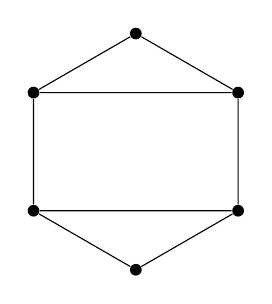
\begin{tikzpicture}[
          every node/.style={circle, fill=black, inner sep=1.5pt},
          edgeLbl/.style={fill=none, inner sep=1.5pt, pos=0.5},
        ]
          \foreach \steps/\text in {1,2,...,6}
          {
            \pgfmathsetmacro{\angle}{(1-\steps)*360/6+90};
            \draw (\angle:1.5 ) node (v\steps) {};
          }
          %%
          \draw (v1) -- (v2) -- (v3) -- (v4) -- (v5) -- (v6) -- (v1) (v2) -- (v6) (v3) -- (v5);
        \end{tikzpicture}
      \end{center}
    \end{minipage}
    \hspace*{\stretch{1}}
    \begin{minipage}{0.45\linewidth}
      \begin{center}
        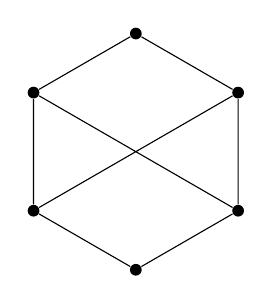
\begin{tikzpicture}[
          every node/.style={circle, fill=black, inner sep=1.5pt},
          edgeLbl/.style={fill=none, inner sep=1.5pt, pos=0.5},
        ]
          \foreach \steps/\text in {1,2,...,6}
          {
            \pgfmathsetmacro{\angle}{(1-\steps)*360/6+90};
            \draw (\angle:1.5 ) node (v\steps) {};
          }
          %%
          \draw (v1) -- (v2) -- (v3) -- (v4) -- (v5) -- (v6) -- (v1) (v2) -- (v5) (v3) -- (v6);
        \end{tikzpicture}
      \end{center}
     \end{minipage}
    \vspace*{\stretch{1}}
  \end{ex*}

  \pagebreak
\end{document}
